\section{Testing}
\subsection{Allgemeine Begriffe}
\begin{itemize}
	\item Definition: Programm mit der Absicht ausführen, Fehler zu finden. 
	\item Durch das Testen kann die Korrektheit eines Programms nicht bewiesen werden!
	\item Mit Testen kann nur die Anwesenheit von Bugs bewiesen werden, aber nicht die Abwesenheit. 
	\item Erster Bug: 1947 wurde eine Motte im Relais eines Mark II Aiken Rechners entdeckt.
\end{itemize}

\subsubsection{Wahrscheinlichkeit von Fehlern}
\begin{minipage}{12cm}
Je mehr Fehler gefunden werden, desto höher ist die Wahrscheinlichkeit weiterer Fehler.
\end{minipage}
\begin{minipage}{6cm}
	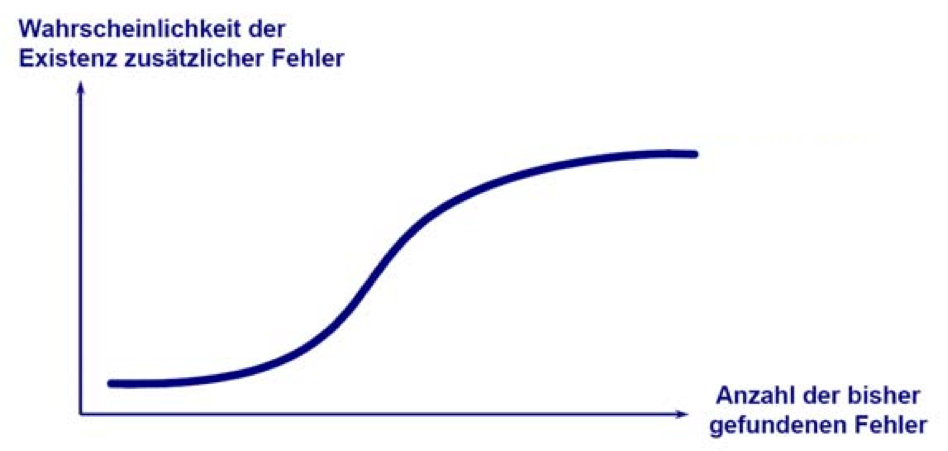
\includegraphics[width=6cm]{images/fehler_wkeit.png}	
\end{minipage}

\begin{multicols}{2}
	\subsubsection{Verifikation \& Validierung}
	\textbf{Validierung:}\\
	\textit{"{}Are we building the right product?"}\\
	Überprüft das Produkt ob es die Anforderungen des Auftraggebers erfüllt.\\
	\textbf{Verifikation:}\\
	\textit{"{}Are we building the product right?"}\\
	Überprüft ob die erstellte Software funktioniert.\\
	
	\subsubsection{Testen \& Debuggen}
	\textbf{Ziel des Testing:} \\
	Aufzeigen, dass Fehler existieren.\\
	\textit{"{}Jeder gefundene Bug ist ein Gold Nugget"}\\
	\textbf{Ziel des Debugging:} \\
	Durch Testing gefundene Fehler lokalisieren und beheben.
	
\end{multicols}

\begin{multicols}{2}	
\subsubsection{Anforderungen an Softwaretests}
	\begin{minipage}{12cm}
	\begin{itemize}
			\item Geplant $\rightarrow$ Testplan erstellen
			\item Systematisch $\rightarrow$ Testspezifikationen erstellen
			\item Festgehalten $\rightarrow$ Testprotokoll erstellen
			\item Reproduzierbarkeit:
			\begin{itemize}
				\item Wissen, was getestet wurde
				\item Unabhängig von testender Person
			\end{itemize}
			\item Automatisierung, wenn möglich
			\item Testspezifikationen laufend erweitern,\\
			Regressionstests
		\end{itemize}
	\end{minipage}
		\begin{minipage}{10cm}
			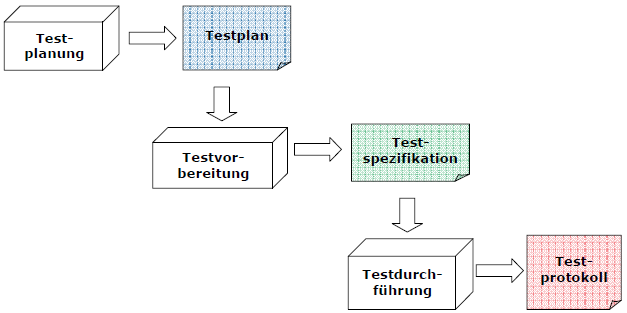
\includegraphics[width=10cm]{images/sofwaretest.png}
		\end{minipage}
\end{multicols}

\begin{multicols}{2}
	\subsubsection{Massnahmen zur Softwareprüfung}
	\begin{itemize}
		\item Dynamische Prüfung
		\begin{itemize}
			\item Testing
			\item Dynamische Analyse
		\end{itemize}
		\item Statische Prüfung
		\begin{itemize}
			\item Metrikanalyse
			\item Code Reviews
		\end{itemize}
	\end{itemize}
	
	\subsubsection{Arten von Tests}
	\begin{itemize}
		\item Funktionale Tests
		\item Nicht-Funktionale Tests
		\begin{itemize}
			\item Leistungstests
			\item Usability Tests
			\item ...
		\end{itemize}
	\end{itemize}
\end{multicols}

\pagebreak
\subsection{Testmethoden}
\subsubsection{Blackbox Tests}
	Tests ohne Kenntnis der inneren Struktur;\\

\textbf{Äquivalenzklassen:} \\
\begin{minipage}{15cm}
Wertebereich, für welche das Programm voraussichtlich das gleiche Verhalten zeigt. \\
Methodik: 1 Testcase pro Äquivalenzklasse \\
Beispiel: Quadratische Gleichung; Determinante $<0$ ; $=0$ ; $>0$ \\
\end{minipage}
\begin{minipage}{4cm}
	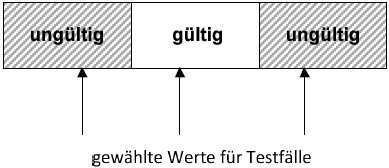
\includegraphics[width=4cm]{images/aequivalenzklasse.png}
\end{minipage}

\textbf{Grenzwertanalyse:} \\
\begin{minipage}{12cm}
Fehler liegen oft an Grenzen zulässiger Eingabewertbereiche. \\
Methodik: Testfälle auf Grenzen und knapp daneben \\
\end{minipage}
\begin{minipage}{4cm}
	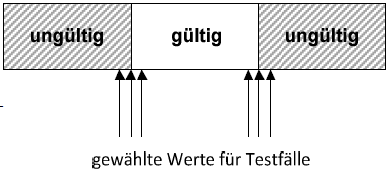
\includegraphics[width=4cm]{images/grenzwertanalyse.png}
\end{minipage}

\textbf{Zustandsbasiertes Testing:} \\
Beispiel Stack: \\
Zustände: Stack leer, Stack halb-voll, Stack voll \\
Testfälle: Element hinzufügen, Element entfernen

\subsubsection{Whitebox Tests}
\begin{minipage}{13cm}
Tests mit Kenntnis der inneren Struktur;\\
Whitebox-Test werden mittels Kontrollfluss-Graphen durchgeführt. \\
Jedes Statement entspricht Knoten.\\
Zweige, stellen Schleifen und Verzweigungen dar, verbinden Knoten. \\
Der Test wird so ausgelegt, dass die Überdeckung (Coverage) möglichst gut ist. (Test der Überdeckung mit Dynamic Analyzer)
\end{minipage}
\begin{minipage}{5.5cm}
	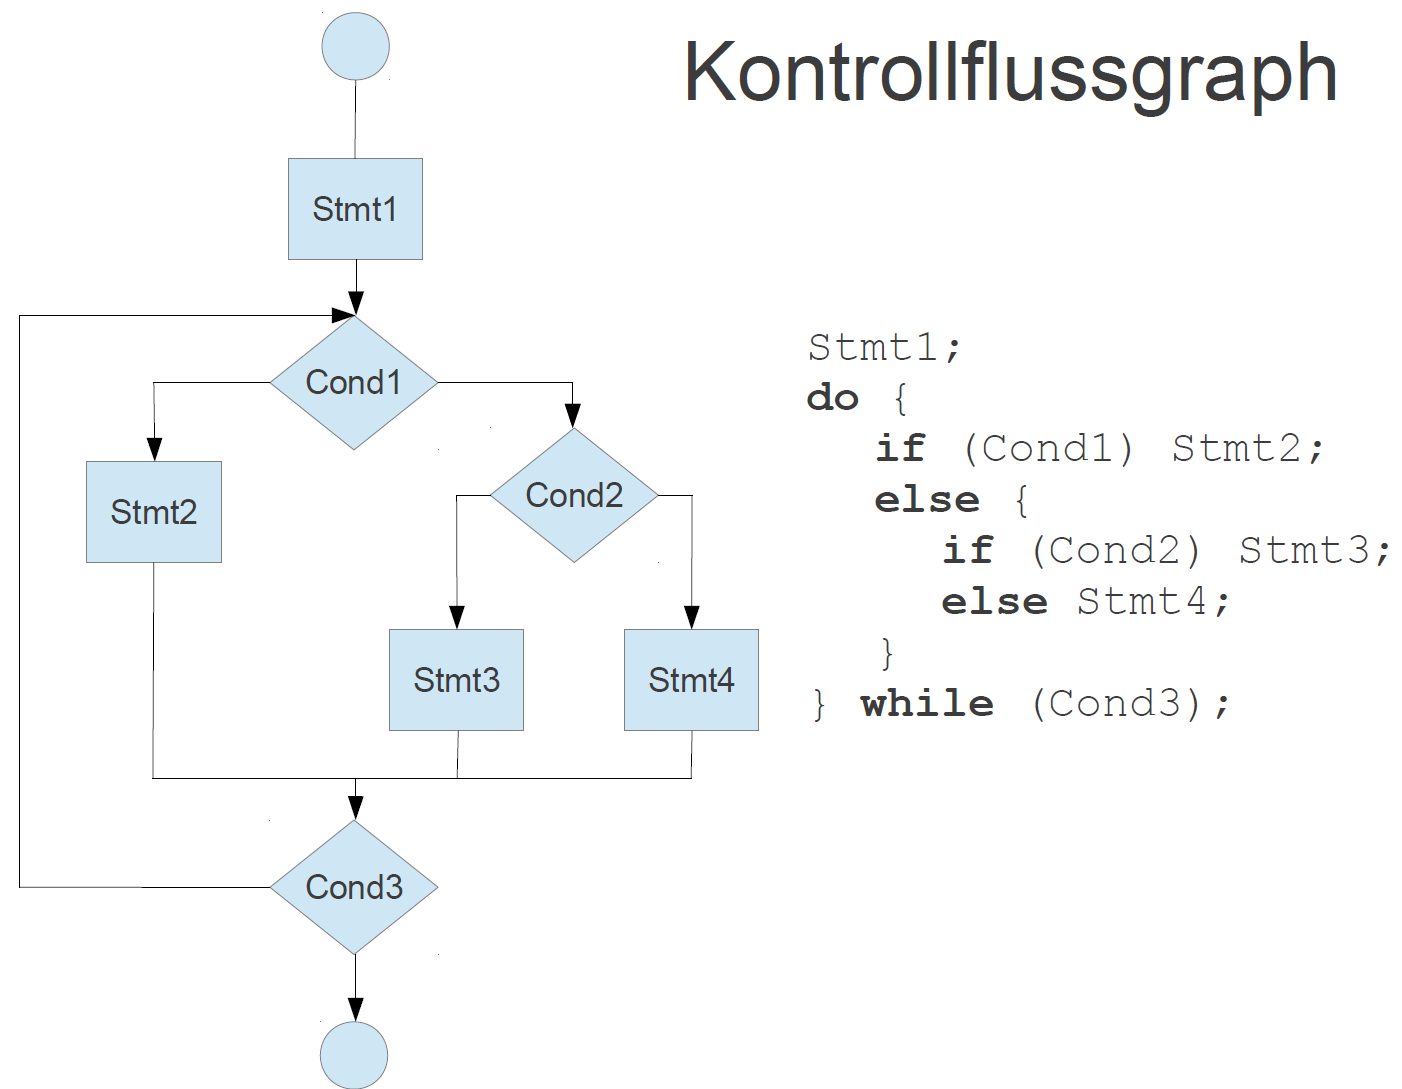
\includegraphics[width=5.5cm]{images/kontrollflussgraphen.png}
\end{minipage}

\begin{itemize}
	\item Anweisungsüberdeckung (statement coverage)
			\begin{itemize}
				\item Prozentualer Anteil der Anweisungen welche im Test ausgeführt werden
				\item 100\% Anweisungsüberdeckung ist Minimum
			\end{itemize}
	\item Zweigüberdeckung (branch coverage)
			\begin{itemize}
				\item Prozentualer Anteil der Zweige welche durchlaufen werden
				\item 100\% Zweigüberdeckung $\Rightarrow$ 100\% Anweisungsüberdeckung
			\end{itemize}
	\item Bedingungsüberdeckung
			\begin{itemize}
				\item Verschiedene Kombinationen testen bei zusammengesetzten Bedingungen
				\item mind. 1x true/false durchlaufen
			\end{itemize}
	\item Pfadüberdeckung (path coverage)
			\begin{itemize}
				\item Prozentualer Anteil der Pfade welche im Test durchlaufen werden
				\item Ein Pfad ist möglicher Weg durch Kontrollgraphen
			\end{itemize}
	\item Funktionsüberdeckung
			\begin{itemize}
				\item \textit{"{}Tut es das, was der Kunde spezifiziert hat?"}
				\item 1 Szenario pro Use Case 
				\item Blackbox Tests
			\end{itemize}
\end{itemize}

\subsection{Testwerkzeuge}
\begin{tabular}{ll}
	Blackbox: & FIT \\
	Whitebox: & xUnit
\end{tabular}


\subsection{Automatisiertes Testing}
\textbf{Vorteile:}
\begin{itemize}
	\item Wiederholbarkeit (Regressionstests möglich)
	\item Eindeutige Spezifikationen (Testcode ist Programmcode)
\end{itemize}	
\textbf{Nachteile:}
\begin{itemize}
	\item Mehr Code zu schreiben und zu pflegen
	\item Testcode ist Programmcode: Wird überhaupt das Richtige getestet?
\end{itemize}

\subsection{Unit-Test}
\subsubsection{Konzept}
\begin{minipage}{10.5cm}
	\begin{itemize}
		\item Test einer Komponente (Unit)
		\item Testen der Schnittstelle der Unit
		\item automatisch wiederholbar
		\item mittels Unit-Test-Frameworks \\
		Frameworks: Programmgerüst in welches das Anwendungsprogramm eingebettet wird. Die Funktionen der Unit werden aus dem Framework heraus aufgerufen, sogennantes Hollywood-Prinzip:\\
		\textit{"{}Don't call us, we'll call you"}
	\end{itemize}
\end{minipage}
\begin{minipage}{9cm}
	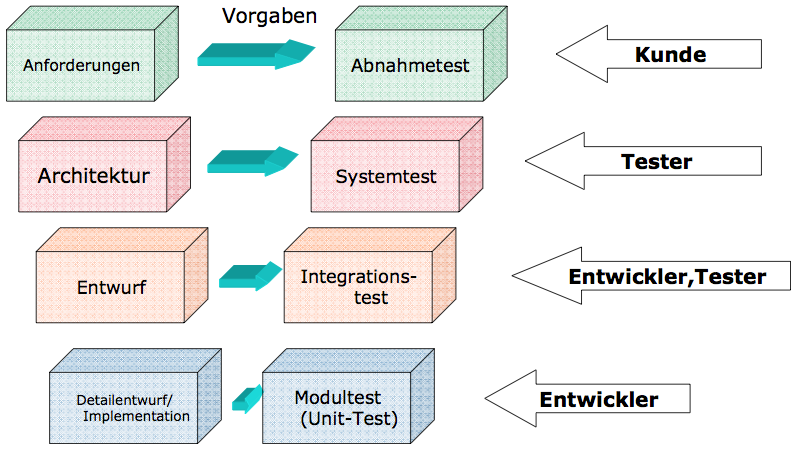
\includegraphics[width=9cm]{images/wer_testet.png}
\end{minipage}

\subsubsection{Arbeitsweise}
\begin{itemize}
	\item Spezielle, möglichst einfache Testfunktion mit Zusicherungen
	\item Test-Run endet mit OK oder FAILED
\end{itemize}

\subsubsection{Vorteile}
\begin{itemize}
	\item Tests sind aufgeteilt, pro Klasse eine Testklasse
	\item Innerhalb der Datei in Testfunktion und Testsuite
	\item Testprotokollausgabe möglich 
\end{itemize}

\subsubsection{Unit-Test mittels CPPUNIT}
\begin{minipage}{15cm}
	\begin{itemize}
		\item Assert-Anweisung, vergleicht Soll mit Ist
		\item Test-Runner Programm das die Test-Funktionen nacheinander ausführt
		\item Testklasse, selbstgeschriebene Klasse die vom Testcase erbt
		\item Testfunktion, enthält Assert-Anweisungen
		\item Testsuite, fasst Testfunktionen zusammen
		\item Testfixture Bereitstellung und Abbau einer Testumgebung
		\item Beispiel im Anhang
	\end{itemize}
\end{minipage}
